\paragraph{Часть 2}
\begin{center}
    \begin{tabular}{|c|l|l|l|l|}
        \hline
        Device              & Interface & IP Address   & Mask          & Default Gateway \\
        \hline
        \multirow{2}{*}{R1} & Fa0/0     & 192.168.1.1  & 255.255.255.0 & N/A             \\
        \cline{2-5}
        ~                   & S0/1/0    & 192.168.2.1  & 255.255.255.0 & N/A             \\
        \hline
        \multirow{2}{*}{R2} & Fa0/0     & 192.168.3.1  & 255.255.255.0 & N/A             \\
        \cline{2-5}
        ~                   & S0/1/0    & 192.168.2.2  & 255.255.255.0 & N/A             \\
        \hline
        PC1                 & Fa0       & 192.168.1.10 & 255.255.255.0 & 192.168.1.1     \\
        \hline
        PC2                 & Fa0       & 192.168.3.10 & 255.255.255.0 & 192.168.3.1     \\
        \hline
    \end{tabular}
\end{center}

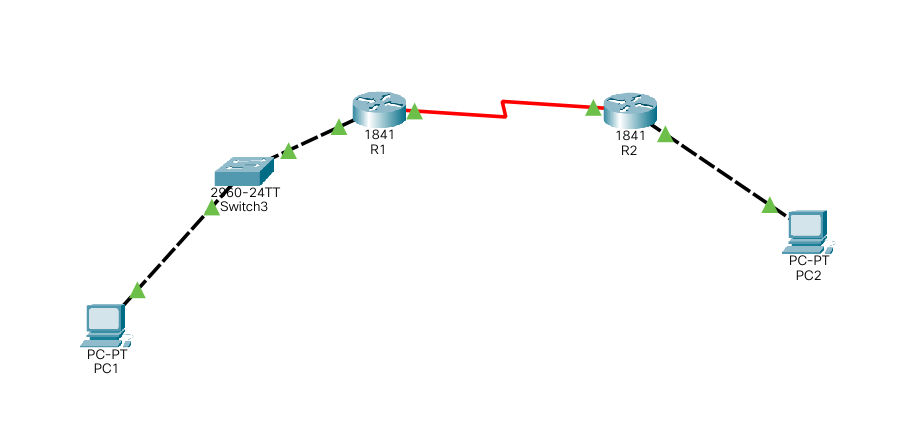
\includegraphics[width=0.9\textwidth]{resources/topology2}

В итоге получилось 3 подсети.
В подсети 1, 3 находятся PC, которые связываются роутерами.
Роутеры коммуницируют между собой в подсети 2.

\LstinputlistingPlain{resources/ping13}{}
